% ============================================================
% GENERAL SEMANTICS: The Virology of Semantic Reactions (English edition)
% + Supplement: School as a factory of injections
%
% SocioCyberneering Inc. — 2026
% XeLaTeX + polyglossia
% Шрифты: Liberation Serif (основной), Montserrat (заголовки/обложка)
% ============================================================
\documentclass[13pt,a4paper]{article}

\usepackage{fontspec}
\usepackage{polyglossia}
\setmainlanguage{english}

\setmainfont{Liberation Serif}
\setsansfont[Scale=0.98]{Liberation Sans}
\setmonofont{DejaVu Sans Mono}[Scale=0.85]
\newfontfamily\montserrat[Path=./fonts/,Extension=.ttf,UprightFont=*-Regular,BoldFont=*-Bold,ItalicFont=*-Regular,BoldItalicFont=*-Bold]{MontserratStatic}

\usepackage{geometry}
\geometry{margin=2.5cm, top=3cm, bottom=3cm}

\usepackage{xcolor}
\usepackage{hyperref}
\usepackage{enumitem}
\usepackage{booktabs}
\usepackage{array}
\usepackage{tabularx}
\usepackage{parskip}
\usepackage{microtype}
\usepackage{graphicx}
\usepackage{titlesec}
\usepackage{setspace}
\usepackage{nameref}
\usepackage{mdframed}
% ---- схемы в стиле «Доска Мерсера» ----
\usepackage{needspace}
\usepackage{pdfpages}
\usepackage{tikz}
\usetikzlibrary{arrows.meta,positioning,calc,backgrounds,fit,shapes.geometric,decorations.pathreplacing}
\definecolor{board}{HTML}{F6EFDD}
\newcommand{\ttl}{\montserrat\bfseries\footnotesize}
\newcounter{scheme}
\newenvironment{scheme}[2]{%
  \par\Needspace{#2}\vspace{0.9em}%
  \noindent{\montserrat\bfseries\small\color{sce-gold}\refstepcounter{scheme}DIAGRAM \thescheme\ \textbullet\ #1}\par
  \vspace{-0.2em}\noindent\textcolor{sce-gold}{\rule{\linewidth}{0.8pt}}\par\vspace{0.4em}\nopagebreak
  \begin{center}\small
}{%
  \end{center}\vspace{0.4em}%
}
\tikzset{
  card/.style={draw=sce-black, line width=1pt, rounded corners=2pt, align=center,
    inner sep=5pt, font=\small, text=sce-black},
  cb/.style={card, fill=bg-blue,  draw=sce-blue},
  cg/.style={card, fill=bg-green, draw=sce-green},
  cr/.style={card, fill=bg-red,   draw=sce-red},
  cy/.style={card, fill=bg-gold,  draw=sce-gold},
  cw/.style={card, fill=white},
  thread/.style={sce-red, line width=1.2pt},
  arr/.style={-{Stealth[length=3mm,width=2.4mm]}, line width=1.4pt, sce-black},
  arrr/.style={-{Stealth[length=3mm,width=2.4mm]}, line width=1.6pt, sce-red},
  arrg/.style={-{Stealth[length=3mm,width=2.4mm]}, line width=1.6pt, sce-green},
  arrd/.style={-{Stealth[length=3mm,width=2.4mm]}, line width=1.2pt, dash pattern=on 4pt off 3pt, sce-grey},
  pin/.style={circle, fill=sce-red, draw=sce-black, line width=0.4pt, inner sep=1.7pt},
}
\newcommand{\boardbg}{%
  \begin{scope}[on background layer]
    \fill[rounded corners=4pt, fill=board, draw=sce-grey, line width=0.6pt]
      ([shift={(-5mm,-5mm)}]current bounding box.south west) rectangle
      ([shift={(5mm,5mm)}]current bounding box.north east);
  \end{scope}}


% ---- глоссарий: термины с якорями и кликабельными ссылками ----
% \term{КОД}{перевод} → [КОД] (перевод) — кликабельно, прыгает в глоссарий
% \termdef{КОД}{перевод} → определяет якорь в глоссарии
\newcommand{\term}[2]{%
  \hyperref[glossary:#1]{%
    \texttt{\textcolor{sce-blue}{[#1]}}%
  }%
  \,{\footnotesize\textcolor{sce-grey}{[#2]}}%
}
% краткий вариант без перевода (когда перевод уже ясен из контекста)
\newcommand{\termr}[1]{%
  \hyperref[glossary:#1]{\textbf{\texttt{\textcolor{sce-blue}{[#1]}}}}%
}
% якорь определения в глоссарии
\newcommand{\termdef}[1]{\phantomsection\label{glossary:#1}}

% красные кавычки: \kav{слово} → 'слово' красным
\newcommand{\kav}[1]{\textcolor{sce-red}{'#1'}}

% ---- цвета SCE ----
\definecolor{sce-blue}{HTML}{154360}      % чернильный синий — механизм/нейтраль
\definecolor{sce-gold}{HTML}{9A7D0A}      % бронзово-золотой — диалог/цитата
\definecolor{sce-red}{HTML}{7B241C}       % тёмно-красный — опасность/предупреждение
\definecolor{sce-grey}{HTML}{2D3748}      % графитовый — вспомогательный
\definecolor{sce-green}{HTML}{145A32}     % тёмно-зелёный — факт/антивирус/решение
\definecolor{sce-black}{HTML}{0D0D0D}     % почти чёрный — основной текст заголовков

\hypersetup{
  colorlinks=true,
  linkcolor=sce-black,
  urlcolor=sce-blue,
}

% ---- стиль заголовков ----
\titleformat{\section}
  {\montserrat\large\bfseries\color{sce-black}\addfontfeatures{LetterSpace=5}}
  {\thesection.}{0.8em}{}[\vspace{-0.3em}\textcolor{sce-gold}{\rule{\linewidth}{0.6pt}}]

\titleformat{\subsection}
  {\montserrat\normalsize\bfseries\color{sce-blue}}
  {\thesubsection.}{0.6em}{}

\titleformat{\subsubsection}
  {\sffamily\small\bfseries\color{sce-grey}}
  {\thesubsubsection.}{0.5em}{}

% ---- фоновые цвета для боксов (светлые) ----
\definecolor{bg-blue}{HTML}{EBF5FB}
\definecolor{bg-gold}{HTML}{FEF9E7}
\definecolor{bg-red}{HTML}{FDEDEC}
\definecolor{bg-green}{HTML}{EAFAF1}

% ---- box-окружения — левая полоса + фон ----
% mechbox — СИНИЙ — механизм, определение, нейтральный анализ
\newenvironment{mechbox}[1]{%
  \vspace{0.9em}
  \begin{mdframed}[
    linecolor=sce-blue, linewidth=4pt,
    topline=false, rightline=false, bottomline=false,
    backgroundcolor=bg-blue,
    innerleftmargin=12pt, innerrightmargin=10pt,
    innertopmargin=8pt, innerbottommargin=8pt,
    skipabove=0pt, skipbelow=0pt
  ]
  \noindent{\montserrat\normalsize\bfseries\color{sce-blue}#1}\par\vspace{4pt}%
  \ignorespaces
}{%
  \end{mdframed}
  \vspace{0.6em}
}

% dialogbox — ЗОЛОТОЙ — цитата, пример из жизни, диалог
\newenvironment{dialogbox}[1]{%
  \vspace{0.9em}
  \begin{mdframed}[
    linecolor=sce-gold, linewidth=4pt,
    topline=false, rightline=false, bottomline=false,
    backgroundcolor=bg-gold,
    innerleftmargin=12pt, innerrightmargin=10pt,
    innertopmargin=8pt, innerbottommargin=8pt,
    skipabove=0pt, skipbelow=0pt
  ]
  \noindent{\montserrat\normalsize\bfseries\color{sce-gold}#1}\par\vspace{4pt}%
  \ignorespaces
}{%
  \end{mdframed}
  \vspace{0.6em}
}

% warnbox — КРАСНЫЙ — опасность, предупреждение, атака
\newenvironment{warnbox}[1]{%
  \vspace{0.9em}
  \begin{mdframed}[
    linecolor=sce-red, linewidth=4pt,
    topline=false, rightline=false, bottomline=false,
    backgroundcolor=bg-red,
    innerleftmargin=12pt, innerrightmargin=10pt,
    innertopmargin=8pt, innerbottommargin=8pt,
    skipabove=0pt, skipbelow=0pt
  ]
  \noindent{\montserrat\normalsize\bfseries\color{sce-red}#1}\par\vspace{4pt}%
  \ignorespaces
}{%
  \end{mdframed}
  \vspace{0.6em}
}

% factbox — ЗЕЛЁНЫЙ — антивирус, инструмент, решение, факт
\newenvironment{factbox}[1]{%
  \vspace{0.9em}
  \begin{mdframed}[
    linecolor=sce-green, linewidth=4pt,
    topline=false, rightline=false, bottomline=false,
    backgroundcolor=bg-green,
    innerleftmargin=12pt, innerrightmargin=10pt,
    innertopmargin=8pt, innerbottommargin=8pt,
    skipabove=0pt, skipbelow=0pt
  ]
  \noindent{\montserrat\normalsize\bfseries\color{sce-green}#1}\par\vspace{4pt}%
  \ignorespaces
}{%
  \end{mdframed}
  \vspace{0.6em}
}

% ============================================================
\begin{document}

% ---- COVER ----
\thispagestyle{empty}
\begin{titlepage}
\centering
\vspace*{3cm}

{\montserrat\bfseries\small\addfontfeatures{LetterSpace=12}\color{sce-black}
G E N E R A L \ S E M A N T I C S}

\vspace{0.4em}
{\montserrat\bfseries\footnotesize\addfontfeatures{LetterSpace=8}\color{sce-black}
T H E \ S C I E N C E \ O F \ H U M A N \ E V A L U A T I O N S}

\vspace{1.8em}
\textcolor{sce-gold}{\rule{0.4\textwidth}{0.6pt}}
\vspace{1.2em}

{\montserrat\fontsize{32}{38}\selectfont\bfseries\color{sce-black}
The Virology\\[0.2em]
of Semantic\\[0.2em]
Reactions}

\vspace{1.4em}
\textcolor{sce-gold}{\rule{0.3\textwidth}{0.4pt}}
\vspace{1.6em}

{\montserrat\bfseries\normalsize\addfontfeatures{LetterSpace=4}\color{sce-black}
A supplement to general semantics}

\vspace{0.5em}
{\small\color{sce-black}\itshape
Includes: The Virology of Evaluations~--- School}

\vfill

\textcolor{sce-gold}{\rule{0.5\textwidth}{0.3pt}}
\vspace{0.8em}

{\montserrat\bfseries\small\addfontfeatures{LetterSpace=8}\color{sce-black}
S O C I O C Y B E R N E E R I N G}

\vspace{0.2em}
{\montserrat\bfseries\footnotesize\addfontfeatures{LetterSpace=5}\color{sce-black}
I N C .}

\vspace{0.6em}
{\small\color{sce-black} 2026 \quad|\quad English edition \quad|\quad GPL-3.0}

\vspace{0.4em}
{\footnotesize\color{sce-black}
\href{https://sociocyber.site}{sociocyber.site} \quad|\quad
\href{https://git.sociocyber.site}{git.sociocyber.site} \quad|\quad
\href{https://github.com/sociocyber1}{github.com/sociocyber1}}

\end{titlepage}

\newpage
\tableofcontents
\newpage

% ============================================================
%  PART I — The Virology of Semantic Reactions
% ============================================================

\newpage
\begin{center}
\vspace*{1cm}
\textcolor{sce-gold}{\rule{0.5\textwidth}{0.4pt}}\\[0.8em]
{\montserrat\Large\bfseries\addfontfeatures{LetterSpace=3}\color{sce-black}
PART I}\\[0.4em]
{\montserrat\large\bfseries\addfontfeatures{LetterSpace=5}\color{sce-grey}
V I R O L O G Y}\\[0.2em]
{\montserrat\normalsize\bfseries\addfontfeatures{LetterSpace=3}\color{sce-grey}
of semantic reactions}\\[0.8em]
\textcolor{sce-gold}{\rule{0.5\textwidth}{0.4pt}}
\vspace{1cm}
\end{center}

\section{Note~--- version 0.1}

This document is not finished. It is published early because it may contain something
important that, as far as I can tell, has not been noticed before. It probably contains
errors of various kinds: in the evaluations, in my \kav{maps} of \kav{maps}, in what I
named \kav{something}, and in what I \kav{observed}-\kav{experienced} to a greater or lesser
degree. Some sections will be changed, with explanations, graphics and pictures added and,
where possible, real examples (if you have any, share them and we will add them).

\subsection{Do not use me to cause harm!}

I do not want you to use these materials deliberately and knowingly for malicious,
destructive ends, such as profiting from people or dulling their minds with something
\kav{pre-scientific}.

For now this document is something like an analysis of wars and of the problems in our
evaluations. Something is clearly wrong, and I am trying to understand it.

\subsection{Injections from me~--- beware!}

I allowed myself some reasoning in the introduction; it may not be that useful.
Be careful with my evaluation. I may have chosen not the most useful name in the section
\kav{The IFD disease}~--- the first term seems to contain some error.
You will need to look at your problem from different points of view and different sciences,
and take into account not only the neuro-evaluative environment but also microbiology and
the external and internal environments.

\subsection{Double-check me!}

I hope you are not like Sherlock Holmes, drawing conclusions hastily, without checking your
hypotheses and evidence. Traces and clues can be forged; inductions and deductions will be
wrong. The conclusions will be false. The map is rigged or wrong.

\begin{warnbox}{No jump to conclusions!}
I have given a general \kav{map}. I may be wrong.\\
Your \kav{Experience 1} and my \kav{Experience 2} do not repeat exactly.\\
Where there is no controlled experiment, it is most likely rubbish, not science.
\end{warnbox}

\section{Introduction}

Welcome to the \textbf{Virology of human evaluations} and of the semantic reactions to them!

This research is carried out within the SocioCyberneering project and within
\textit{SocioCyberneering: Architecture Design Pre-Definitions For Safety-Live-Behavior-In-Semantic-Reaction-Environments}.

Mass disasters and worse things horrified me and made me look for answers.
To bring human relations into symbiosis with the planet, without wars, poverty and politics,
we must find the causes of wars themselves, the sources of \kav{hatred} itself and of general
recklessness.

\begin{mechbox}{Key questions}
Which viruses exist in our \kav{biological software}?\\[0.3em]
How are they transmitted?\\[0.3em]
Do \kav{symbols} transform us \kav{biochemically} and change our \kav{neuro-evaluative transactions}?\\[0.3em]
What \kav{semantic diseases} reach us from the books of the past?\\[0.3em]
What exactly do they read there, the \kav{ministers of war} and the \kav{kings and presidents}?
\end{mechbox}

Relying on symbols is like driving through a green light while running over pedestrians.
The symbol said: go. The observation was skipped. The result: a person is hit.

Reports are symbols. Books are symbols. An old manuscript is a symbol.
Direct observation is lost; you cannot simply look into the past and check.

\begin{dialogbox}{Example~--- how symbols lead to war}
The king wrote: \kav{avenge our people and conquer France}.\\
That does not mean anyone of his actually died.\\
He could have made a false entry to push the prince into war.\\
Names can differ: \kav{only godless heretics live there}.\\[0.4em]
The map replaced the territory.\\
War is the consequence.
\end{dialogbox}

\section{The IFD disease}

In his book Wendell Johnson wrote:

\begin{dialogbox}{Wendell Johnson~--- on the IFD disease}
Ideals in the IFD pattern reach upward in three respects: they are vaguely defined;
they are highly valued; and in their definition they are poorly matched to reality.\\[0.4em]
A person's inability to recognize their own achievements leads to a feeling of frustration,
which in turn leads to (a)~a sense of some degree of inadequacy and (b)~subsequent
reactions, from aggression to plain despondency and loss of initiative.\\[0.4em]
The IFD disease: from idealism to frustration and then to demoralization.\\
Its prevalence approaches the pandemic.
\end{dialogbox}

\begin{scheme}{The IFD cycle after Wendell Johnson}{7.5cm}
\begin{tikzpicture}
  \node[cy, text width=4.4cm] (i) at (0,2.6)     {\textbf{Idealism}\\ideal is vague, high, poorly matched to reality};
  \node[cr, text width=4.4cm] (f) at (5.2,-1.2)  {\textbf{Frustration}\\no achievements seen, sense of inadequacy};
  \node[cr, text width=4.4cm, line width=1.6pt] (d) at (-5.2,-1.2) {\textbf{Demoralization}\\aggression, despondency, loss of initiative};
  \draw[arrr] (i) -- (f);
  \draw[arrr] (f) -- (d);
  \draw[arrr] (d) -- node[above left=-1pt,font=\footnotesize\itshape,text=sce-red]{a new, even less attainable ideal} (i);
  \node[font=\montserrat\bfseries\normalsize, text=sce-red, align=center] at (0,0) {IFD};
  \foreach \n in {i,f,d} \node[pin] at (\n.north west) {};
  \boardbg
\end{tikzpicture}
\end{scheme}

Worries, fears and forebodings make up a large share of our personal maladjustments.
We experience \textbf{evaluative fear}: facts themselves do not torment us morally as much
as we do it ourselves with our evaluations of those facts, and with the devils we conjure
out of thin air.

The IFD disease is less an ailment of individuals than a reflection of the semantic forces
acting on them. We easily \kav{catch semantic sores}.

\begin{mechbox}{How are semantic sores transmitted?}
A hint lies in the inability of maladjusted people to put their difficulties into words
in a way that allows an effective answer.\\[0.3em]
This points to \textbf{language}: to the fact that destructive factors are present in the
structure of our common language.\\[0.3em]
Alfred Korzybski analyzed this problem in \textit{Science and Sanity},\\
and, in a more condensed form, Samuel Hayakawa in \textit{Language in Action}.
\end{mechbox}

\section{Bypassing the \kav{cortex}. The role of the amygdala in madness}

\begin{mechbox}{\termr{E.A.Alert}~--- Emygdala Alert}
An attack in which an attacker, or a chance event, switches a person into
\kav{fight-or-flight} mode by stimulating the brain through words, phrases, clothing,
status, premises, objects and accessories.\\[0.4em]
\textbf{Methods:}
\begin{itemize}
  \item Hanging labels on you
  \item Threatening
  \item Hinting at a threat, a debt, unconscious assumptions
  \item Suggesting: \kav{you are the label, and so you feel this}
  \item Speaking in a stern tone to raise your cortisol level~--- to make you afraid
\end{itemize}
\end{mechbox}

For example: \kav{I can see you are nervous}~--- the attacker deliberately tries to provoke
this semantic reaction, to make you say something you will regret.

The goal: \textbf{switch off the prefrontal cortex}:
\begin{enumerate}
  \item Let the pituitary release cortisol
  \item Put the amygdala into action first
  \item Stop the signal from reaching the cortex
  \item Re-route the signals so that the person's voice is recognized as a threat
\end{enumerate}

As a result you are left with no way to carry out an adequate analysis.

\begin{scheme}{Cortex bypass: the fast path against the slow path}{9cm}
\begin{tikzpicture}
  \node[cy, text width=6.2cm] (tr) at (0,0) {\textbf{Trigger}\\word \textbullet\ tone \textbullet\ status \textbullet\ label};
  \node[cr, text width=4.6cm] (am) at (-4.2,-2.5) {\textbf{Thalamus $\to$ Amygdala}\\fast path, milliseconds};
  \node[cb, text width=4.6cm] (co) at (4.2,-2.5) {\textbf{Thalamus $\to$ Cortex}\\slow path};
  \node[cr, text width=4.6cm] (ko) at (-4.2,-5.0) {\textbf{Cortisol}\\\kav{fight or flight}};
  \node[cw, dashed, text width=4.6cm] (an) at (4.2,-5.0) {\textbf{Analysis}\\too late~--- switched off};
  \node[cr, text width=8.4cm, line width=1.6pt] (ea) at (0,-7.4) {\termr{E.A.Alert}\\\textbf{reaction without analysis}};
  \draw[arrr] (tr.south west) ++(0.6,0) -- (am.north);
  \draw[arrd] (tr.south east) ++(-0.6,0) -- (co.north);
  \draw[arrr] (am) -- (ko);
  \draw[arrd] (co) -- (an);
  \draw[arrr] (ko.south) -- ++(0,-0.5) -| ([xshift=-2cm]ea.north);
  \draw[arrd] (an.south) -- ++(0,-0.5) -| ([xshift=2cm]ea.north);
  \node[font=\footnotesize\itshape, text=sce-red] at (0,-3.7) {the cortex gets the signal later};
  \node[pin] at (tr.north west) {}; \node[pin] at (am.north west) {}; \node[pin] at (co.north west) {};
  \node[pin] at (ko.north west) {}; \node[pin] at (an.north west) {}; \node[pin] at (ea.north west) {};
  \boardbg
\end{tikzpicture}
\end{scheme}

\begin{warnbox}{Rumination~--- the amygdala takes control}
Recalling an event, a dialogue or a quarrel, you can switch into \kav{fight-or-flight} mode
again, just because of an \kav{image} in your head.\\[0.4em]
You replay dialogues in a loop: \kav{how could I have answered so that they would regret it}.\\
Your cortisol is up again. 5 minutes, 1 trigger. You are drained.\\[0.4em]
\textbf{Tell yourself:} \kav{This is not analysis. Stop. Rumination again.
The amygdala has taken control of my semantic reactions to this event.
How can I respond adequately?}
\end{warnbox}

\subsection{The destructive effect of alcohol. IFD is contagious. How the sick affect children and adults}

With this problem you can literally \kav{catch} IFD from a person, and even \kav{infect}
others. Alcohol disrupts the gut microbiome, so proper nourishment does not reach the
neurons. When the amygdala repeatedly puts you into \kav{fight-or-flight} mode and releases
cortisol, you cannot evaluate adequately.

\begin{warnbox}{Never leave a child with a person who has IFD}
Otherwise the child will take on their illnesses. Constant attacks will drive the child to
suicidal thoughts.\\[0.3em]
A child in \kav{fight-or-flight} mode sees the world as extremely dangerous: places seem
empty, frightening, dark, and people not to be trusted.\\[0.3em]
IFD plus alcohol clearly makes the problem worse. In time come shouting and family
violence.
\end{warnbox}

\subsection{War is justified by a hormone, not by logic}

When it comes to peace negotiations, you cannot reach agreement if something puts you and
the person across from you into \kav{fight-or-flight} mode. The amygdala dictates the
semantic reactions.

To push people to fight, they are first switched into \kav{fight-or-flight} mode; having
taken control of the amygdala, the necessary destructive semantic reactions are dictated
through radio, TV, music, symbols and posters.

\begin{warnbox}{The unthinkable part}
Children in kindergartens and schools are trained into these inadequate semantic reactions,
with the default setting that killing for kings is normal,\\
and by building aggression toward images, signs and symbols that distinguish one group
from another.\\[0.3em]
This is a serious danger.
\end{warnbox}

\section{Semantic reaction injection}

\begin{mechbox}{Definition}
\texttt{Semantic-Reaction-Injection [SRI]}\\
\textit{Russian: Инъекция Семантических Реакций [ИСР]}\\[0.4em]
The deliberate or accidental introduction of map-labels into a person's evaluative system,
changing their semantic reactions and bypassing conscious analysis.
\end{mechbox}

\section{Modules}

\begin{mechbox}{\termr{SRI.DS}~--- S.R.I. Detection System}
An intrusion detection system that analyzes individuals' semantic reactions and their
systemic statements for suspicious verbal activity, to spot dangerous tendencies in
evaluations and to forecast incidents.
\end{mechbox}

\begin{mechbox}{CAPTCHA}
A test used to tell humans from logical machines, applied to prevent automatic inadequate
maps and other actions through evaluation.
\end{mechbox}

\section{Attacks}

Viruses are used to replace your responding semantic reactions with an unnatural, inadequate
order of the process of abstracting.

\begin{mechbox}{\termr{SM}~--- Semantic Malware}
Harmful language that damages individuals. Kinds include: intensional maps not checked
against the territory; cruel language; religious viruses; trojan maps that carry far-reaching
unconscious assumptions.
\end{mechbox}

\begin{mechbox}{\termr{MAP Spoofing} / [MPS]~--- MAP Spoofing}
An attack in which the attacker draws false map-messages, supplying inadequate terms and
generalizing conclusions-labels to change semantic reactions and our unconscious evaluations,
re-wiring neural network activations.
\end{mechbox}

\begin{mechbox}{\termr{BruF}~--- Brute Force}
A method of unconscious attack in which the attacker tries every possible combination of
words and phrases until finding the one that provokes you into an inadequate responding
semantic reaction, in order to say afterwards that you started it yourself.
\end{mechbox}

\begin{mechbox}{\termr{SREx}~--- S.R. Exploit}
A language subroutine, hormone-code, map, evaluation, image or analogy that uses
vulnerabilities in the process of abstracting-evaluating to perform unauthorized actions,
with complete takeover of control over the evaluation.
\end{mechbox}

\begin{mechbox}{\termr{SR.Script}~--- S.R. Scripting}
In the context of speeches: the process of writing talking points to provoke the desired
responding semantic reactions. The recipient interprets sound and builds maps in the head
that barely correspond to the real territory.
\end{mechbox}

\begin{mechbox}{\termr{SRI.S}~--- S.R. Injection by Status}
Defining you by status, by your position in life, and injecting evaluations and
\kav{correct} views. First a label is hung on you, then the needed self-evaluation-map is
inserted, turning you into an insecure individual.
\end{mechbox}

\begin{mechbox}{\termr{SRI-Priority}~--- S.R. Injection by Priority (attack on the nervous system)}
Exploits the sense of guilt. A stern tone, a frown, being told \kav{your place} in words
automatically switches you into Emygdala Alert mode.\\
You give priority to evaluations that are not your own, simply because they were spoken
sternly.
\end{mechbox}

\begin{mechbox}{\termr{SRI-DA}~--- S.R.I. Dictionary Attack}
An attack using a pre-built list of words (a dictionary) to provoke inadequate semantic
reactions. It moves the individual into Emygdala Alert.
\end{mechbox}

\begin{mechbox}{\termr{MTS}~--- Map Terminology Spoofing}
A process in which the attacker substitutes the terminology of a map to hide a personal
interest. A map with the wrong terminology is passed on as an objective one.
\end{mechbox}

\begin{mechbox}{\termr{GRB}~--- Gormon S.R. Backdoor}
A hormonal program-language code conditioned by the language environment from birth:
mechanisms that bypass the usual means of proper abstracting\\
and gain unauthorized access to the system.
\end{mechbox}

\begin{mechbox}{\termr{CSRF}~--- Cross-S.R. Request Forgery}
An attack in which the attacker makes an individual perform an unwanted action under
supposedly someone else's responsibility. Using semantic injections, the person then uses
special phrases to shed personal responsibility.
\end{mechbox}

\begin{mechbox}{\termr{DDoP}~--- Distributed Denial of People}
A large number of demands to achieve \kav{success} when it is clearly impossible at that
time: limited resources of food, water and sleep. Overstimulation with words. Overloading
with labels.
\end{mechbox}

\begin{mechbox}{\termr{CRS}~--- Cross ReEvulation S.R. Scripting}
An attack in which the attacker inserts a harmful script (unconscious assumptions,
evaluations) into an evaluation that other individuals accept as given, with no evidence
and no checks.
\end{mechbox}

\begin{mechbox}{\termr{MITM}~--- Man-in-the-Middle}
An attack in which a person, deliberately or unconsciously, intercepts and changes the
evaluations passing between two parties during communication, without their knowledge.\\
Implemented through the Emygdala Alert attack.
\end{mechbox}

\section{Common data transmission errors in communication}

Communication between people resembles a game of broken telephone.
Each handover from person to person distorts the original data.

\begin{mechbox}{\termr{EDC}~--- Extentional Data Corruption}
The process of converting extensional data into an intensional, unmeasurable form that is
not available for understanding without special training in observing, asking questions,
clarifying facts and experimenting, making extensional data unavailable when it is passed on
in teaching, books and schools.
\end{mechbox}

\begin{mechbox}{\termr{AS.RL}~--- Abstract Semantic-Reaction Layer}
\kav{Encryption} protocols in documents, contracts and so-called confidentiality policies
(a.k.a. the small print) that keep orientation intensional and break the transmission of
extensional data. Word-injectors with no physical evidence or measurement.
\end{mechbox}

\section{Aberrant behavior}

Behavior that results from accumulated semantic attacks: rumination, aggression, anxiety,
inability to hold a dialogue, avoidance, abstract fears. It is not a sign of weakness but of
the lack of tools for working with the evaluative environment.

\section{Checking the map against the territory}

\begin{mechbox}{\termr{Rootkit}~--- Hidden conclusions}
Unconscious factors of the external and internal environment, hidden and designed to keep
permanent access. Rootkits may change evaluations through physiological processes, making
them hard to detect with standard Aristotelian methods.
\end{mechbox}

Checking the map against the territory is the only means of defense:
\begin{itemize}
  \item Ask: \textit{\kav{is this a fact or an evaluation?}}
  \item Lower the level of abstraction: \textit{\kav{what exactly happened?}}
  \item Allow for uncertainty: \textit{\kav{I do not know enough}}
  \item Do not jump to conclusions~--- \texttt{No jump to conclusions!}
\end{itemize}

% ============================================================
%  PART II — The Virology of Evaluations: School
% ============================================================

\newpage
\begin{center}
\vspace*{1cm}
\textcolor{sce-gold}{\rule{0.5\textwidth}{0.4pt}}\\[0.8em]
{\montserrat\Large\bfseries\addfontfeatures{LetterSpace=3}\color{sce-black}
PART II}\\[0.4em]
{\montserrat\large\bfseries\addfontfeatures{LetterSpace=5}\color{sce-grey}
V I R O L O G Y}\\[0.2em]
{\montserrat\normalsize\bfseries\addfontfeatures{LetterSpace=3}\color{sce-grey}
of evaluations~--- School}\\[0.4em]
{\small\itshape\color{sce-grey}
A supplement to \kav{The Virology of Semantic Reactions} v\,0.1}\\[0.8em]
\textcolor{sce-gold}{\rule{0.5\textwidth}{0.4pt}}
\vspace{1cm}
\end{center}

\section{Introduction~--- school as a transmission environment}

School is not a neutral environment.\\
It is the \textbf{first mass transmission point of semantic viruses}.

A child arrives with an open system of abstracting. They have no settled maps yet. They are
an \textit{observer}. Over 12 years school systematically replaces observation with a
\textbf{label}.

\begin{warnbox}{Key observation}
School is not necessarily malicious.\\
It is a system in which \textbf{the teachers are themselves infected} and pass on what they
have.\\[0.3em]
\termr{GRB} $\to$ the teacher's shout $\to$ the pupil's \termr{GRB} $\to$ the shout of their
own children.\\[0.3em]
A chain. Not a conspiracy. A virus.
\end{warnbox}

\section{The grading system~--- \termr{MAP Spoofing} on an industrial scale}

\subsection{What a grade is at school}

A school grade is a number from 1 to 5 (or a letter, or a percentage).
It is a \textbf{map}. It describes \textit{something} about the child's behavior at a
specific moment.

But the school system passes it on differently:

\begin{mechbox}{How a grade is passed on~--- the chain of abstractions}
\textbf{Level 0 (event):} the child could not retell the text at 2:30 pm on Tuesday\\
\textbf{Level 1 (grade):} \kav{2} in the register\\
\textbf{Level 2 (generalization):} \kav{studies badly}\\
\textbf{Level 3 (personality):} \kav{lazy}, \kav{stupid}, \kav{incapable}\\
\textbf{Level 4 (forecast):} \kav{will never amount to anything}\\[0.4em]
Each level up is \textbf{farther from the territory}.\\
School works at levels 3--4. That is \termr{MAP Spoofing}.
\end{mechbox}

\begin{scheme}{Ladder of abstraction: from event to label}{9cm}
\begin{tikzpicture}
  \node[cg, text width=2.65cm, anchor=north west] (a0) at (0,0)      {\ttl LEVEL 0 \\[1pt] \textbf{Event}\\could not retell the text};
  \node[cb, text width=2.65cm, anchor=north west] (a1) at (3.1,-0.9) {\ttl LEVEL 1 \\[1pt] \textbf{Grade}\\\kav{2} in the register};
  \node[cy, text width=2.65cm, anchor=north west] (a2) at (6.2,-1.8) {\ttl LEVEL 2 \\[1pt] \textbf{Generalization}\\\kav{studies badly}};
  \node[cr, text width=2.65cm, anchor=north west] (a3) at (9.3,-2.7) {\ttl LEVEL 3 \\[1pt] \textbf{Personality}\\\kav{lazy}, \kav{stupid}};
  \node[cr, text width=2.65cm, anchor=north west, line width=1.6pt] (a4) at (12.4,-3.6) {\ttl LEVEL 4 \\[1pt] \textbf{Forecast}\\\kav{will never amount to anything}};
  \foreach \a/\b in {a0/a1,a1/a2,a2/a3,a3/a4}
    \draw[thread] (\a.east) ++(0,-0.2) to[out=0,in=180] (\b.west);
  \foreach \n in {a0,a1,a2,a3,a4} \node[pin] at (\n.north west) {};
  \draw[arr] (0,-7.0) -- node[below=2pt,font=\footnotesize\itshape] {distance from the territory grows} (15.4,-7.0);
  \node[font=\footnotesize\bfseries, text=sce-green, anchor=south west] at (0,-6.95) {TERRITORY};
  \node[font=\footnotesize\bfseries, text=sce-red, anchor=south east] at (15.4,-6.95) {MAP};
  \draw[decorate,decoration={brace,amplitude=5pt,mirror}, sce-red, line width=1.2pt]
     (9.3,-6.4) -- (15.4,-6.4) node[midway,below=6pt, font=\footnotesize\bfseries, text=sce-red] {};
  \node[font=\footnotesize\bfseries, text=sce-red] at (12.35,-8.1) {school works here \termr{MAP Spoofing}};
  \boardbg
\end{tikzpicture}
\end{scheme}

\subsection{Why this is \termr{MAP Spoofing}}

\termr{MAP Spoofing} is an attack in which the system gives a \textbf{false map-label}
instead of a description of the real event. The school grade as a label:
\begin{itemize}
  \item Does not describe \textit{what exactly} did not work
  \item Does not explain \textit{why}
  \item Does not contain a \textit{tool} for fixing it
  \item Is hung on the child's \textbf{personality}
\end{itemize}

\begin{dialogbox}{Example~--- a real chain}
Teacher (aloud, in front of the class):\\
\kav{Another fail. You are not trying at all.}\\[0.3em]
What happened: the child could not retell the text.\\
What was said: \texttt{[you] = [not trying]}~--- an evaluation of the person.\\
What stays with the child: a map of themself as \kav{the one who does not try}.\\[0.3em]
Territory: no method for working with a text.\\
Map: \textit{lazy}.
\end{dialogbox}

\section{\termr{SRI} in the classroom~--- injections of grades}

\subsection{Public humiliation as \termr{E.A.Alert}}

When a teacher reads grades aloud in front of the class,
it is an \textbf{\termr{E.A.Alert}} for the child with a low grade.

\begin{mechbox}{The trigger mechanism}
1. The teacher says the name and the fail in front of everyone.\\
2. The class looks. Laughter. Or silence, which is worse.\\
3. Amygdala: a threat to social status is a threat to survival.\\
4. Cortisol rises.\\
5. The cortex switches off. Analysis is impossible.\\
6. The child is in \kav{fight-or-flight} mode.\\[0.3em]
In this state they \textbf{cannot learn}. But the lesson goes on.
\end{mechbox}

\subsection{Repeated \termr{GRB}~--- forming a reflex}

If \termr{E.A.Alert} in the classroom repeats regularly, the child develops a \termr{GRB}:

\begin{mechbox}{\termr{GRB} in the school context}
\textbf{Trigger:} a knowledge-check situation (test, question at the board, retelling)\\
\textbf{Hormonal response:} cortisol $\to$ amygdala $\to$ threat mode\\
\textbf{Behavior:} stupor, forgetting, stammering, aggression, withdrawal\\
\textbf{The child's map of themself:} \kav{I cannot}\\[0.3em]
Later, the adult in any checking situation\\
gets the same cortisol. \textbf{Although there is no threat.}\\[0.3em]
This is \termr{GRB}. The school backdoor. For life.
\end{mechbox}

\subsection{\termr{SRI-Priority}~--- a stern tone as a tool}

A teacher with an authoritative tone is \termr{SRI-Priority}:
the child accepts the teacher's map \textbf{without checking}, even if the map is false.
The result is \textbf{intensional orientation}: the child lives not by fact but by label.

\section{The virology of grades~--- classification of school attacks}

\begin{mechbox}{Table~--- attacks in the school environment}
\begin{tabularx}{\linewidth}{@{} l X @{}}
\toprule
\textbf{Code} & \textbf{Description of the attack at school} \\
\midrule
\termr{MAP Spoofing} &
  A grade as a label of the personality instead of a description of a specific action. \\[0.3em]
\termr{E.A.Alert} &
  Public announcement of a grade. The class as an audience of the threat. \\[0.3em]
\termr{GRB} &
  Forming a hormonal backdoor: a checking situation equals a threat. A lifelong reflex. \\[0.3em]
\termr{SRI-Priority} &
  The teacher's stern tone as authority. Intensional orientation. \\[0.3em]
\termr{SRI} &
  Injection: \textit{\kav{you must}, \kav{all normal children can}, \kav{you should be ashamed}}. \\[0.3em]
\termr{DDoP} &
  Overload: homework + tests + demands + grades + parents. \\[0.3em]
\termr{EDC} &
  Rote learning: observation and understanding replaced by wording from the textbook. \\[0.3em]
\termr{Rootkit} &
  A hidden preset: \textit{\kav{a good grade = you are a good person}}. \\[0.3em]
\termr{CRS} &
  \textit{\kav{Peter can, and you cannot}}. Someone else's evaluation as the standard. \\
\bottomrule
\end{tabularx}
\end{mechbox}

\section{Laziness does not exist~--- \termr{MAP Spoofing} by the name of \kav{laziness}}

\begin{warnbox}{Central thesis}
The label \texttt{[ LAZINESS ]} is \textbf{\termr{MAP Spoofing}}.\\
It describes not the territory but \textit{the absence of a map in the observer}.\\[0.3em]
When a teacher (or parent) says \kav{is being lazy}\\
it means: \textit{I do not see the real cause. I am using a label.}
\end{warnbox}

Behind the \texttt{[ LAZINESS ]} label in the school context there is always one of these:

\begin{factbox}{What is hidden behind the label~--- the territory}
\begin{itemize}
  \item \textbf{No method}~--- the child does not know how to work with this type of task. This is \termr{EDC}.
  \item \textbf{No meaning}~--- the link between the task and life is not explained. The brain saves resources.
  \item \textbf{\termr{GRB} is active}~--- cortisol. In threat mode, learning is biologically blocked.
  \item \textbf{Exhaustion~--- \termr{DDoP}}~--- 6 lessons + homework + clubs + anxiety at home.
  \item \textbf{Hidden protest}~--- refusal of what is imposed. A signal of a mismatch.
  \item \textbf{\termr{FEAR OF ERROR}}~--- fear of making a mistake paralyzes action.
\end{itemize}
\end{factbox}

\begin{scheme}{Behind the label [ LAZINESS ]: cause and tool}{10cm}
\begin{tikzpicture}
  \node[cr, text width=2.65cm, line width=1.6pt] (lz) at (0.6,-3.3) {\textbf{[ LAZINESS ]}\\label\\\termr{MAP Spoofing}};
  \foreach \i/\y/\c/\cause/\tool in {
     1/0/cb/{No method}/{show the step: \kav{here is how I do it}},
     2/-1.35/cb/{No meaning}/{show the link to life},
     3/-2.7/cr/{\termr{GRB} is active}/{pause, remove the threat},
     4/-4.05/cy/{Exhaustion \termr{DDoP}}/{cut the excess, give resources},
     5/-5.4/cy/{Hidden protest}/{ask what is wrong},
     6/-6.75/cr/{\termr{FEAR OF ERROR}}/{redefine the mistake}}
  {
    \node[\c, text width=4.0cm] (c\i) at (6.3,\y) {\textbf{\cause}};
    \node[cg, text width=4.9cm] (t\i) at (12.2,\y) {\tool};
    \draw[thread] (lz.east) to[out=0,in=180] (c\i.west);
    \draw[arrg] (c\i.east) -- (t\i.west);
    \node[pin] at (c\i.north west) {};
  }
  \node[font=\ttl, text=sce-grey] at (6.3,1.0) {TERRITORY: the real cause};
  \node[font=\ttl, text=sce-green] at (12.2,1.0) {A TOOL INSTEAD OF A LABEL};
  \boardbg
\end{tikzpicture}
\end{scheme}

\subsection{The chain of passing on the label}

\begin{center}
\begin{tabular}{ccccc}
School & $\to$ & teacher's \termr{GRB} & $\to$ & Label \kav{lazy} \\
$\downarrow$ & & & & $\downarrow$ \\
No method & & & & child's \termr{GRB} \\
$\downarrow$ & & & & $\downarrow$ \\
Child goes home & $\to$ & Mother sees the fail & $\to$ & mother's \termr{GRB} \\
& & $\downarrow$ & & \\
& & Shout & $\to$ & \termr{FEAR OF ERROR} \\
& & $\downarrow$ & & \\
& & \multicolumn{3}{l}{\texttt{[ LAZINESS ]}~--- the label settles in the child's map of themself} \\
\end{tabular}
\end{center}

Neither the teacher nor the mother is aware of the chain. They \textbf{pass on what they
themselves received}.\\
This is a \textbf{virus}.

\begin{scheme}{The infection chain: how the virus is passed around in a circle}{10cm}
\begin{tikzpicture}
  \node[cy, text width=3.6cm] (n1) at (0,3.3)    {\textbf{School}\\grade as a label};
  \node[cr, text width=3.6cm] (n2) at (5.0,1.7)  {\textbf{Teacher}\\\termr{GRB}: pressure, tone};
  \node[cr, text width=3.6cm] (n3) at (5.0,-1.7) {\textbf{Child}\\\termr{E.A.Alert} in class};
  \node[cr, text width=3.6cm] (n4) at (0,-3.3)   {\textbf{Parent at home}\\\termr{GRB}: the fail in the diary};
  \node[cr, text width=3.6cm] (n5) at (-5.0,-1.7){\textbf{Shout}\\instead of a question};
  \node[cr, text width=3.6cm, line width=1.6pt] (n6) at (-5.0,1.7) {\textbf{Child}\\\termr{FEAR OF ERROR}, label \kav{lazy}};
  \draw[arrr] (n1) -- (n2);
  \draw[arrr] (n2) -- (n3);
  \draw[arrr] (n3) -- (n4);
  \draw[arrr] (n4) -- (n5);
  \draw[arrr] (n5) -- (n6);
  \draw[arrr] (n6) -- node[above left=-1pt,font=\footnotesize\itshape,text=sce-red,pos=0.45]{next generation} (n1);
  \node[font=\montserrat\bfseries\normalsize, text=sce-red, align=center] at (0,0) {THE VIRUS\\DOES NOT DIE};
  \foreach \n in {n1,n2,n3,n4,n5,n6} \node[pin] at (\n.north west) {};
  \boardbg
\end{tikzpicture}
\end{scheme}

\section{Rote learning~--- \termr{EDC} as a systemic attack}

\subsection{The EDC mechanism in studying}

\begin{mechbox}{The normal process vs. school rote learning}
\textbf{The normal process of abstracting:}\\
Event (observation) $\to$ Description $\to$ Generalization $\to$ Principle\\[0.4em]
\textbf{School rote learning:}\\
Wording from the textbook $\to$ Memorize $\to$ Reproduce $\to$ Grade\\[0.4em]
Observation is skipped. Understanding is optional.\\
Connection with reality is absent.
\end{mechbox}

\subsection{Example: a poem}

\begin{dialogbox}{A real situation (flashback)}
Assignment: learn a poem by heart.\\
The aim per the curriculum: developing memory and \kav{introduction to culture}.\\[0.4em]
What happens in reality:\\
The child does not understand the text. The words are abstract.\\
There is no method: how do you work with a text you do not understand?\\
Result: rote learning without meaning. Or refusal. Or \termr{GRB}.\\[0.3em]
Label: \texttt{[ LAZINESS ]}.\\
Territory: \textit{no tool for working with the incomprehensible}.
\end{dialogbox}

\subsection{A tool instead of rote learning}

\begin{factbox}{Four steps instead of \kav{learn it by heart}}
1. \textbf{Read the first two lines. Say in your own words what they are about.}\\
   (Extensional observation: what did I understand?)\\[0.3em]
2. \textbf{Find one word you do not understand.}\\
   (Making it concrete: what exactly gets in the way?)\\[0.3em]
3. \textbf{Come up with an image for each line.}\\
   (Link to experience: map $\leftrightarrow$ territory)\\[0.3em]
4. \textbf{Tell it~--- do not repeat it, tell it.}\\
   (Checking understanding, not memory)\\[0.3em]
It takes the same 20 minutes.\\
But the child gets a \textbf{method}, not a fear reflex.
\end{factbox}

\section{Patriotism at school~--- \termr{SR.Script} and \termr{Rootkit}}

\subsection{The formation mechanism}

\begin{mechbox}{Components of \termr{SR.Script} at school}
\textbf{Symbols:} flag, coat of arms, anthem~--- anchors for \termr{E.A.Alert}\\
\textbf{Narrative:} history as a set of correct maps\\
\textbf{Ritual:} the assembly line-up, the minute of silence, \kav{our country is great}\\
\textbf{Grade:} the right answer about the \kav{motherland} = a good grade\\
\textbf{Pressure:} a wrong answer = moral condemnation by the group\\[0.3em]
Result: \termr{Rootkit}, a hidden preset:\\
\textit{\kav{my country is always right}}~--- works without awareness.
\end{mechbox}

\subsection{Why this is a \termr{Rootkit}}

\termr{Rootkit}: hidden assumptions that are \textbf{not noticed} and give \textbf{permanent
access} to evaluations:
\begin{itemize}
  \item Not subjected to checking~--- it is \textit{taken for granted}
  \item Activates automatically on a trigger (flag, anthem, \kav{enemy})
  \item Blocks critical analysis: \textit{\kav{this is betrayal}}
  \item Passed to the next generation through the same rituals
\end{itemize}

\subsection{Parents' aggression~--- a product of the school environment}

When school demands patriotic behavior + grades + results,
it passes \textbf{pressure} on to the parents:

\begin{enumerate}
  \item School: \textit{\kav{your child is not meeting the requirements}}
  \item Parent: \termr{GRB} activates~--- shame, fear, anger
  \item At home: shouting, pressure on the child~--- \textit{\kav{why the fail?}}
  \item Child: \termr{E.A.Alert} + \termr{GRB} $\to$ \termr{FEAR OF ERROR}
  \item Result: the child does not learn better. They learn \textbf{to be afraid}.
\end{enumerate}

\begin{dialogbox}{Key observation}
The parent does not want to cause harm.\\
The parent is themself infected with \termr{GRB} from \textit{their own} school.\\
Shouting is not cruelty. It is \textbf{the only tool}\\
that was handed down to them.\\[0.3em]
School gave no methods~--- it gave \textbf{pressure + a grade}.\\
The parent transmits what they received.\\[0.3em]
The virus has been passed on.
\end{dialogbox}

\section{Consequences~--- the map of the self}

A child who has spent 10--12 years in such a system leaves with a set of maps:

\begin{warnbox}{Maps issued by the school system}
\texttt{[I = my grade]}~--- a person's worth is determined by a number\\
\texttt{[a mistake = danger]}~--- \termr{FEAR OF ERROR} as the basic setting\\
\texttt{[not knowing = shame]}~--- not knowing is not a beginning, it is a failure\\
\texttt{[authority is right]}~--- a map accepted without checking~--- \termr{SRI-Priority}\\
\texttt{[I am lazy/stupid/incapable]}~--- a label accepted as fact\\
\texttt{[thinking is dangerous]}~--- the right answer matters more than honest observation
\end{warnbox}

\subsection{What school did not pass on}

\begin{factbox}{What should have been passed on}
\begin{itemize}
  \item How to work with an incomprehensible text (a method, not rote learning)
  \item How to ask questions (extensional orientation)
  \item How to notice that you do not know, and to count it as a beginning, not a failure
  \item How to check a map~--- \textit{\kav{is this a fact or an evaluation?}}
  \item How to cope with a mistake~--- \textit{\kav{what exactly did not work?}}
  \item How to recognize \termr{E.A.Alert} in yourself and make a pause
\end{itemize}
\textbf{This is General Semantics.}\\
It is not taught, because the system itself runs on \termr{MAP Spoofing}.
\end{factbox}

\section{Antivirus~--- what works}

\subsection{Recognizing the level of abstraction}

\begin{mechbox}{Questions for checking a map}
\textbf{Is this a fact or an evaluation?}\\
\textit{\kav{He is lazy}}~--- an evaluation. \textit{\kav{He did not hand in three assignments}}~--- closer to a fact.\\[0.3em]
\textbf{What exactly happened?}\\
Not \textit{\kav{studies badly}} but: \textit{\kav{in the fractions task he skips the cancelling step}}.\\[0.3em]
\textbf{What tool is needed?}\\
Not \textit{\kav{try harder}} but: \textit{\kav{let us go through this step another way}}.
\end{mechbox}

\subsection{A pause before \termr{GRB}}

\termr{GRB} is hormonal. It cannot be switched off by thought. But you can \textbf{create a pause}.

\begin{factbox}{The pause method}
1. Notice: \textit{\kav{I have cortisol right now. What triggered it?}}\\
2. Name the trigger: \textit{\kav{a fail in the diary}}~--- it is an event, not a catastrophe.\\
3. Separate the event from the evaluation:\\
   \textit{\kav{A fail}}~$\neq$~\textit{\kav{a bad child}}~$\neq$~\textit{\kav{I am a bad parent}}\\
4. Ask a question instead of shouting:\\
   \textit{\kav{What exactly did not work?}}
\end{factbox}

\begin{scheme}{Antivirus: a pause between trigger and reaction}{5cm}
\begin{tikzpicture}
  \node[cr, text width=2.9cm] (a) at (0,0)    {\textbf{Trigger}\\\termr{GRB} fires: cortisol};
  \node[cy, text width=2.9cm] (b) at (3.4,0)  {\textbf{1. Notice}\\\kav{I have cortisol right now}};
  \node[cb, text width=2.9cm] (c) at (6.8,0)  {\textbf{2. Name}\\what exactly set it off};
  \node[cb, text width=2.9cm] (d) at (10.2,0) {\textbf{3. Separate}\\event from evaluation};
  \node[cg, text width=2.9cm, line width=1.6pt] (e) at (13.6,0) {\textbf{4. Ask}\\\kav{what exactly did not work?}};
  \foreach \a/\b in {a/b,b/c,c/d,d/e} \draw[arrg] (\a) -- (\b);
  \node[font=\footnotesize\bfseries, text=sce-green] at (8.5,-1.9) {the pause: the reflex ends here and choice begins};
  \draw[decorate,decoration={brace,amplitude=5pt,mirror}, sce-green, line width=1.2pt] (3.4,-1.2) -- (13.6,-1.2);
  \foreach \n in {a,b,c,d,e} \node[pin] at (\n.north west) {};
  \boardbg
\end{tikzpicture}
\end{scheme}

\subsection{A tool instead of a label~--- three steps}

\begin{factbox}{Three steps instead of the label \kav{laziness}}
\textbf{1. No method $\to$ show the step}\\
Not \textit{\kav{try harder}} but: \textit{\kav{here is how I do it. Try it the same way}}.\\[0.3em]
\textbf{2. No meaning $\to$ show the connection}\\
Not \textit{\kav{you need to know it}} but: \textit{\kav{you need this when...}}.\\[0.3em]
\textbf{3. Fear of error $\to$ redefine the mistake}\\
Not \textit{\kav{wrong again}} but: \textit{\kav{great. Now we know exactly what is off}}.
\end{factbox}

\section{Summary~--- school in the terms of virology}

\begin{warnbox}{The summary map}
\textbf{School as an environment:}\\
A mass transmission point of \termr{GRB}, \termr{MAP Spoofing}, \termr{EDC}, \termr{Rootkit}.\\[0.3em]
\textbf{The mechanism:}\\
A grade as a label of the personality~--- instead of a description of an action.\\
Publicity as \termr{E.A.Alert}~--- instead of a safe environment.\\
Rote learning as \termr{EDC}~--- instead of a method for working with the incomprehensible.\\
Patriotism as \termr{Rootkit}~--- instead of a skill for checking the map.\\[0.3em]
\textbf{The result:}\\
\termr{FEAR OF ERROR}~--- a lifelong reflex.\\
A map of the self as a set of labels accepted without checking.\\[0.3em]
\textbf{Transmission:}\\
Children $\to$ parents (pressure at home).\\
Children $\to$ the next generation (the same \termr{GRB}).\\
The virus does not die. It is passed on.\\[0.3em]
\textbf{Antivirus:}\\
A tool instead of a label. A pause instead of \termr{GRB}.\\
A question instead of a shout. This is General Semantics.
\end{warnbox}

% ============================================================
% GLOSSARY
% ============================================================
\newpage
\section*{Glossary of terms}
\addcontentsline{toc}{section}{Glossary of terms}

Every code in the text is a clickable link to this section.\\
Format: \texttt{[CODE]} \textbf{English term}, then the \textit{Russian term} and a description.

\vspace{0.6em}

\termdef{E.A.Alert}
\noindent\textbf{\texttt{[E.A.Alert]}} \quad \textbf{Emygdala Alert}\\
\textit{Russian:} Тревога амигдалы\\
The amygdala takes control, bypassing the cortex. Fight-or-flight starts from a word, a tone or a status, with no real physical threat. Analysis is blocked.

\vspace{0.5em}
\termdef{GRB}
\noindent\textbf{\texttt{[GRB]}} \quad \textbf{Gormon S.R. Backdoor}\\
\textit{Russian:} Гормональный бэкдор семантических реакций\\
A conditioned hormonal reflex formed by the language environment in childhood. A trigger (a word, a situation, a symbol) releases cortisol automatically, without awareness. Lifelong unless detected.

\vspace{0.5em}
\termdef{SRI}
\noindent\textbf{\texttt{[SRI]} / \texttt{[ИСР]}} \quad \textbf{Semantic-Reaction Injection}\\
\textit{Russian:} Инъекция семантических реакций (ИСР)\\
The deliberate or accidental introduction of map-labels into a person's evaluative system, changing their reactions and bypassing conscious analysis.

\vspace{0.5em}
\termdef{SRI.DS}
\noindent\textbf{\texttt{[SRI.DS]}} \quad \textbf{S.R.I. Detection System}\\
\textit{Russian:} Система обнаружения вторжений\\
Analyzes semantic reactions and statements for suspicious activity, dangerous tendencies in evaluations and incident forecasts.

\vspace{0.5em}
\termdef{SRI-Priority}
\noindent\textbf{\texttt{[SRI-Priority]}} \quad \textbf{S.R. Injection by Priority}\\
\textit{Russian:} Инъекция через авторитет\\
A stern tone, status or a frown makes you accept a map without checking. You give priority to someone else's evaluation simply because it was spoken with authority.

\vspace{0.5em}
\termdef{MAP Spoofing}
\noindent\textbf{\texttt{[MAP Spoofing]} / \texttt{[MPS]}} \quad \textbf{MAP Spoofing}\\
\textit{Russian:} Отравление картой (подмена карты)\\
Supplying a false map-label instead of describing the real event. The classic case: an evaluation of the person instead of a description of a specific action. Works through \termr{EDC}, replacing observation with a label.

\vspace{0.5em}
\termdef{EDC}
\noindent\textbf{\texttt{[EDC]}} \quad \textbf{Extentional Data Corruption}\\
\textit{Russian:} Коррупция экстенсиональных данных\\
Replacing observation (what exactly happened?) with a label or a wording. Rote learning is a typical EDC: words without understanding. An evaluation of the person instead of a description of the action is EDC too.

\vspace{0.5em}
\termdef{Rootkit}
\noindent\textbf{\texttt{[Rootkit]}} \quad \textbf{Rootkit (Hidden conclusions)}\\
\textit{Russian:} Скрытые предустановки\\
Unconscious assumptions that run in the background and give permanent access to evaluations. Example: \kav{a good grade = a good person}. Not noticed, and therefore never checked.

\vspace{0.5em}
\termdef{DDoP}
\noindent\textbf{\texttt{[DDoP]}} \quad \textbf{Distributed Denial of People}\\
\textit{Russian:} Распределённый отказ людям (перегрузка)\\
An overload of demands, tasks and expectations that cannot be met at the moment. It drains resources and blocks learning. School analogue: 6 lessons + homework + clubs + anxiety.

\vspace{0.5em}
\termdef{FEAR OF ERROR}
\noindent\textbf{\texttt{[FEAR\_OF\_ERROR: HIGH]}} \quad \textbf{FEAR\_OF\_ERROR: HIGH}\\
\textit{Russian:} Страх ошибки: высокий\\
A reflex in which a possible mistake blocks action. Formed by repeated \termr{GRB} in checking situations. Result: better not to act than to act wrongly.

\vspace{0.5em}
\termdef{SR.Script}
\noindent\textbf{\texttt{[SR.Script]}} \quad \textbf{S.R. Scripting}\\
\textit{Russian:} Скриптинг семантических реакций\\
Prepared talking points, symbols and rituals that provoke the desired reactions in an audience. Used in propaganda, advertising and school assemblies. Works through \termr{E.A.Alert}.

\vspace{0.5em}
\termdef{SM}
\noindent\textbf{\texttt{[SM]}} \quad \textbf{Semantic Malware}\\
\textit{Russian:} Семантическая малварь\\
Harmful language: intensional maps without checking, cruel language, religious viruses, trojan maps with hidden assumptions.

\vspace{0.5em}
\termdef{BruF}
\noindent\textbf{\texttt{[BruF]}} \quad \textbf{Brute Force}\\
\textit{Russian:} Брутфорс\\
Trying provoking words and phrases until the trigger is found, after which the victim \kav{started it}. The unconscious version is everyday squabbling.

\vspace{0.5em}
\termdef{SREx}
\noindent\textbf{\texttt{[SREx]}} \quad \textbf{S.R. Exploit}\\
\textit{Russian:} Эксплойт семантических реакций\\
A language construction that uses a weakness in the process of abstracting. Complete takeover of the evaluation without awareness of the attack.

\vspace{0.5em}
\termdef{SRI.S}
\noindent\textbf{\texttt{[SRI.S]}} \quad \textbf{S.R. Injection by Status}\\
\textit{Russian:} Инъекция через статус\\
Defining a person by their position, then inserting a \kav{correct} self-evaluation. A tool of suppression through classification.

\vspace{0.5em}
\termdef{SRI-DA}
\noindent\textbf{\texttt{[SRI-DA]}} \quad \textbf{S.R.I. Dictionary Attack}\\
\textit{Russian:} Словарная атака\\
A prepared list of trigger words to move someone into \termr{E.A.Alert}. Dictionaries of hatred and insults are the typical example.

\vspace{0.5em}
\termdef{MTS}
\noindent\textbf{\texttt{[MTS]}} \quad \textbf{Map Terminology Spoofing}\\
\textit{Russian:} Подмена терминологии карты\\
Substituting words in the map to hide a personal interest. \kav{War} becomes \kav{special operation}. \kav{Murder} becomes \kav{neutralization}.

\vspace{0.5em}
\termdef{CSRF}
\noindent\textbf{\texttt{[CSRF]}} \quad \textbf{Cross-S.R. Request Forgery}\\
\textit{Russian:} Подделка запроса между реакциями\\
The attacker makes a person act while shedding responsibility with special phrases. \kav{It's your own fault}. \kav{I warned you}.

\vspace{0.5em}
\termdef{CRS}
\noindent\textbf{\texttt{[CRS]}} \quad \textbf{Cross ReEvulation S.R. Scripting}\\
\textit{Russian:} Перекрёстный скриптинг оценок\\
One person's harmful evaluation is accepted by others without checking. \kav{Peter can, and you cannot}. Someone else's map becomes your own.

\vspace{0.5em}
\termdef{MITM}
\noindent\textbf{\texttt{[MITM]}} \quad \textbf{Man-in-the-Middle}\\
\textit{Russian:} Человек посередине\\
Interception and distortion of evaluations between two parties. Implemented through \termr{E.A.Alert}: while both sides are in threat mode, the middleman controls the transmission.

\vspace{0.5em}
\termdef{AS.RL}
\noindent\textbf{\texttt{[AS.RL]}} \quad \textbf{Abstract Semantic-Reaction Layer}\\
\textit{Russian:} Абстрактный слой семантических реакций\\
\kav{Encryption} protocols in documents, contracts and small print. They keep orientation intensional and break the transmission of extensional data.

% ============================================================
\vspace{3em}
\begin{center}
\textcolor{sce-gold}{\rule{0.5\textwidth}{0.4pt}}\\[0.6em]
{\montserrat\bfseries\small\addfontfeatures{LetterSpace=6}\color{sce-black}
S O C I O C Y B E R N E E R I N G \ I N C .}\\[0.2em]
{\footnotesize\color{sce-black}
\href{https://sociocyber.site}{sociocyber.site} \quad|\quad
GPL-3.0 \quad|\quad 2026}
\end{center}

% ============================================================
%  APPENDIX — Problem-Solving Workbook (Russian original, embedded in full)
% ============================================================
\newpage
\phantomsection
\addcontentsline{toc}{section}{Appendix: Problem-Solving Workbook}
\thispagestyle{empty}
\begin{center}
\vspace*{5cm}
\textcolor{sce-gold}{\rule{0.5\textwidth}{0.6pt}}\\[1.2em]
{\montserrat\large\bfseries\addfontfeatures{LetterSpace=6}\color{sce-black}APPENDIX}\\[1.2em]
{\montserrat\fontsize{24}{30}\selectfont\bfseries\color{sce-black}Problem-Solving\\Workbook}\\[1.2em]
{\montserrat\normalsize\bfseries\color{sce-grey}Six steps from problem to action}\\[1.4em]
\textcolor{sce-gold}{\rule{0.5\textwidth}{0.6pt}}\\[1.4em]
{\small\color{sce-black}A tool instead of a label: a continuation of Parts I and II\\
The workbook follows in full (14 pages)\\
Original: TalkPlus (created August 2023, revised August 2024)}
\end{center}
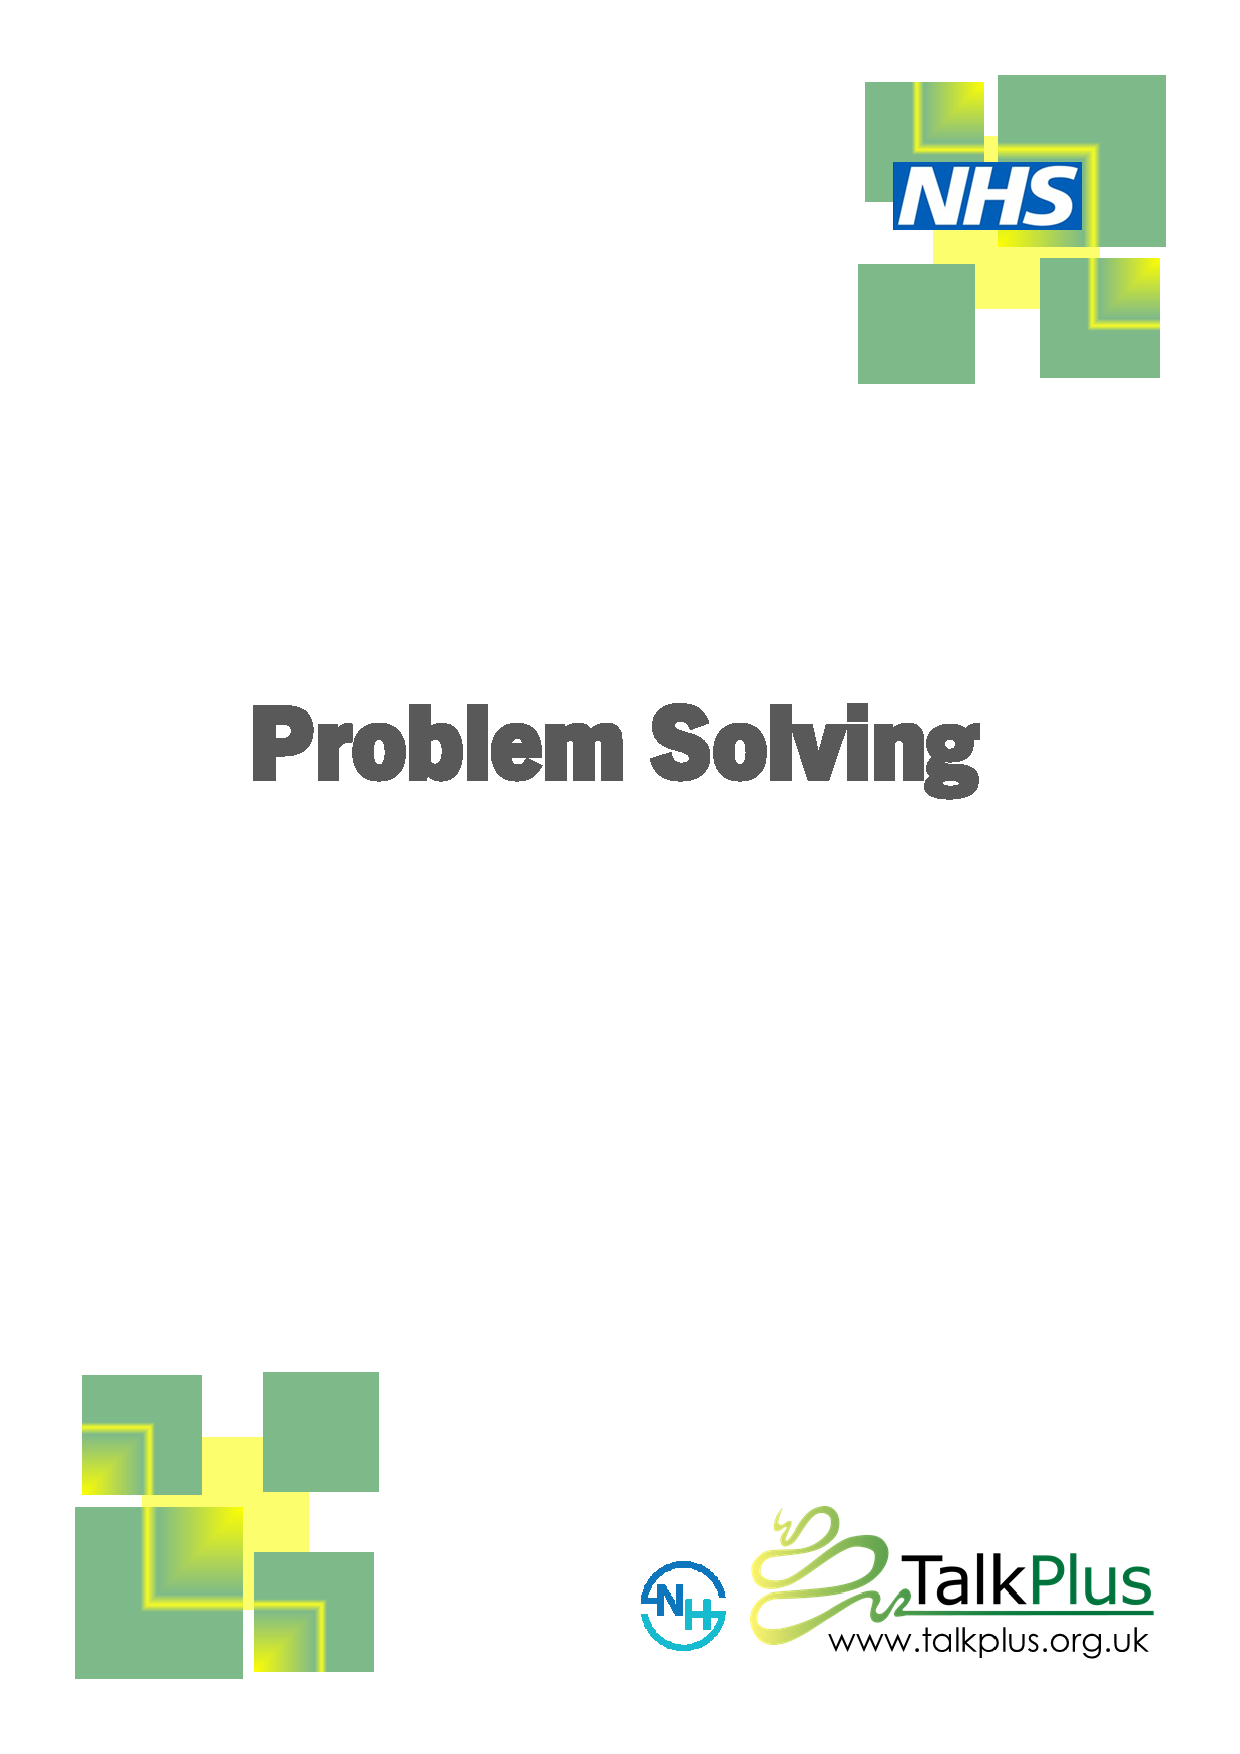
\includepdf[pages=-,pagecommand={\thispagestyle{empty}}]{appendix/problem_solving_en.pdf}

\end{document}
